\documentclass[12pt]{article}

% Margins
\usepackage[letterpaper, top=1in, bottom=1in, left=.5in, right=.5in]{geometry}

% For prettier tables
\usepackage{array}

\usepackage{graphicx}

\usepackage{caption}

\usepackage{float}

% For code
\usepackage{courier}
\usepackage{listings}
\lstset{ mathescape }
\lstset{basicstyle=\ttfamily\footnotesize,breaklines=true}

\usepackage{hyperref}

% Change Font
\usepackage[sfdefault]{roboto}  %% Option 'sfdefault' only if the base font of the document is to be sans serif
\usepackage[T1]{fontenc}

% For double spacing
\usepackage{setspace}

\usepackage[english]{babel}
\usepackage[utf8]{inputenc}
\usepackage{fancyhdr}

\pagenumbering{arabic}

\pagestyle{fancy}
\rhead{Jimmy Hickey}

\lhead{Progress Report II}


%opening
\title{
Computer Corrected Color Blindness: Progress Report II
}
\author{Jimmy Hickey}



\begin{document}
\maketitle
\doublespacing

\begin{abstract}
Many people suffer from color deficient vision; though they learn to cope, they still have many issues distinguishing between colors. In this research, I propose a combination of machine learning algorithms that can help eliminate some of the problems faced by these individuals. As a prototype, specialized data with intentional color blind issues is generated, transformed, and used to train the system. The colors in these images are then segmented using k-means clustering. A supervised neural network is trained to predict these clusters and applied to other images. The image will then be analyzed and corrected if neighboring clusters are found to be conflicting. After correcting, the image will be more color blind friendly.

\end{abstract}

\section{Introduction}

Color blindness is a deficiency in a person's color vision. A color blind person will often confuse different colors that a person with normal vision would not have trouble distinguishing. The most common type of color blindness is red-green, followed by blue-yellow, and the rare full lack of color vision. Red-green color blindness effects "as many as 8 percent of men and 0.5 percent of women with Northern European ancestry." (National Eye Institute) The effects of color blindness range from minor disruptions such as choosing a mismatched outfit to more major difficulties such as discerning between the colors of traffic lights.
There is no cure for color blindness, however there exist some methods to alleviate symptoms. 

One popular solution to color blindness is specialized glasses. The company enchroma sells a variety of these glasses. Color vision starts in the cones of the eye, of which people have three varieties: green, red, and blue. These detect and distinguish between different wavelengths of light; however, in the eye of a color blind person, this discrimination is not always made properly. The enchroma glasses filter out the overlapping wavelengths, making distinctions (particularly between red and green) clearer. These glasses range from \$349 to \$429 without prescriptions and are not ``intended to help pass color blindness tests for occupational purposes." (enchroma) Additionally, they (enchroma brand) are not useful to people with blue-yellow color blindness. A more permanent solution is currently being tested as well.

There is experimental gene therapy that has produced promising results in animals. In one study squirrel monkeys, which are naturally red-green color blind, were made able to perceive differences in the two colors after treatment. These animals were monitored and ``retained their new tricolor sensory capacity for more than two years." (MIT Technology Review). Additionally, there have been no detected harmful side effects from the treatment; four more animals have been successfully treated since. These auspicious trials suggest that there may be a permanent fix to color blindness in the near future; however, gene therapy is often prohibitively expensive, costings hundreds of thousands of dollars per patient. A short-term, cheap solution to some of the issues faced by the color blind is needed. 

The burgeoning field of computer vision lends itself perfectly to this problem. Much work has been done in the area of feature recognition. Projects like Google's deep dream and work in robotic vision are some of the wide applications of computer vision. Computers' abilities to analyze images is greatly enhancing. These methods can be used as the small, cheap fix to some color blind issues. A first step would be to examine images.

Instead of recognizing complex features, a machine needs only to examine the colors in an image. With appropriate knowledge of the problem domain, it should be able to diagnose whether there is areas of the image that may cause issues for the color blind. For example, given a set of color blind tests, it would be able to tell which slides a color blind person would have trouble with. This process can then be incrementally furthered.

\begin{enumerate}
	\item The system can mark all problem areas.
	\item The system can fix the problem areas without losing too much of the context of the image.
	\item The system can perform the preceding actions on a video.
	\item The system can perform the preceding actions on a live video feed.
\end{enumerate}

For the scope of this project, the first and second object will be addressed.

Unlike the glasses, the machine is not dealing with the light itself, but how it is displayed. Thus, this could be easily expanded to support all of the common types of color blindness. 


\section{Hypothesis}
A system can be trained to identify and resolve areas of potential color blind confusion in images.


\section{Methods}

\subsection{Data Creation}
\subsubsection{Image Creation}
Initially, it was planned to use standard Ishihara Color Test plates, such as those used by eye doctors, as the data for this experiment. See figure \ref{fig:ishi} for an example.

\begin{figure}[H]
	\centering
	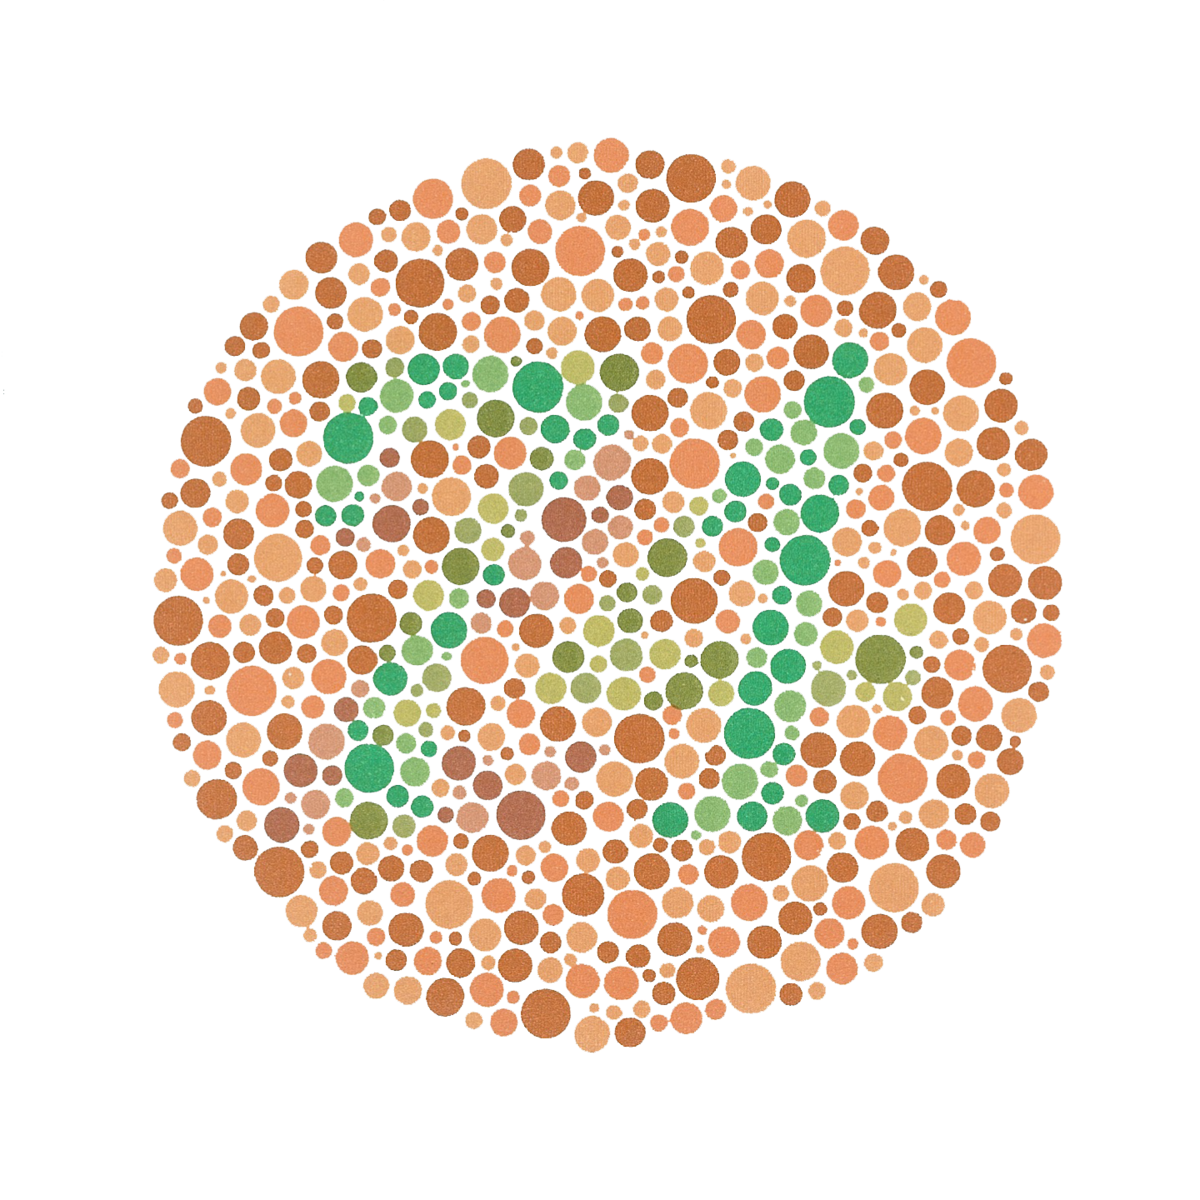
\includegraphics[width=0.25\textwidth]{img/Ishihara}
	\caption{A red-green Ishihara color blind plate.}
	\captionsetup{font={footnotesize,bf,it}}
	\caption*{\href{https://en.wikipedia.org/wiki/Ishihara\_test}{https://en.wikipedia.org/wiki/Ishihara\_test}}
	\label{fig:ishi}
\end{figure}

However, this afforded little control of the data. The learning process would rely on only the Ishihara samples publicly available online. 

Instead of this, new data was generated for the sake of this experiment. This allows for a wider range of data to be created and manipulated to help the system learn more color combinations. The data created using Adobe Illustrator. A background was chosen and then a foreground image was drawn. The colors of the background and foreground were tweaked until a red-green color blind person started having trouble distinguishing between the two. Figure \ref{fig:data1} shows pink sailboat on a gray background.

\begin{figure}[H]
	\centering
	
\includegraphics[width=0.25\textwidth]{img/data2.png}
	\caption{A sample data point.}
	\label{fig:data1}
\end{figure}

For a color blind person (particularly red-green color blind), it may be very difficult to discriminate between the background and foreground. This process will be continued to create a plethora of color combinations such as blue-purple, brown-red, orange-yellow, red-green, etc. These color combinations will then be altered and repeated. For example, dark blue and dark purple will be used in one image a lighter tint of each color will be used in another.

Issues with the devised data creation system will be explored in the Future Improvements section.

\subsubsection{Image Translation}
The image data needs to be represented in a more quantitative format while still maintaining the information stored in the picture. Namely, the infomration to retain is the color and location of each pixel. Thus, the x and y position will be stored as well as the blue, green, and red values for each pixel. Table \ref{table:1} shows a few rows of the data table representing the sailboat image from figure \ref{fig:data1}. 

\begin{table}[H]
	\centering
	\begin{tabular}{ c c c c c}
		x & y & B & G & R \\\hline 
		0 & 0 & 205 & 205 & 205 \\  
		0 & 0 & 205 & 205 & 205 \\
		0 & 0 & 205 & 205 & 205 \\    
		&  & \vdots &  &  \\ 
		57 & 116 & 217 & 184 &233\\
		&  & \vdots &  &  \\ 
		0 & 0 & 205 & 205 & 205 \\		
	\end{tabular}
	\caption{Image representation of sail boat picture}
	\label{table:1}
\end{table}

\subsection{Color Detection}
Unsupervised learning algorithms including pattern recognition will be used to solve this problem. Differences in color could be detected in each image. Currently, k-means clustering is being used to find distinct trends in the images. Since each image is created to depict a combination of two colors, the k-means algorithm is instructed to dichotimize the data.

The k-means algorithm works as follows:
\begin{enumerate}
\item Determine how many clusters the data will be separated into. For this project, two clusters will be used.
\item Randomly select a mean for each cluster.
\item Classify each piece of data according to each mean.
\item Use these new classifications to recompute the mean of each cluster.
\item Repeat 3-4 until the clusters converge (that is, they do not change more than a threshhold between iterations).
\end{enumerate}

Using this algorithm on the sail boat image shown in figure \ref{fig:data1} sucessfully bisects the data into clusters. One cluster of pixels has been changed to all black to clearly represent the difference:

\begin{figure}[H]
	\centering
	
\includegraphics[width=0.25\textwidth]{img/testtest.png}
	\caption{The k-means algorithm segmenting an image.}
	\label{fig:kmeans1}
\end{figure}



It is expected that the system will identify issues with the red and green more so than the blue since it will be given data for a red-green color blind person. Though k-means is sensitive to outliers, since multiple images will be created for each color combination, local maxima convergence will, hopefully, be avoided. 

\subsection{Color Correction}

One simple correction method that could be employed is through the use of edge detection. Once the system is properly trained to determine problem areas in images, an edge could be detected. Tracing this area with a thin black line would offer a visible separation between the two competing colors, while trying not to lose the information stored in the image.

Another possible correction procedure is to change the colors of the image itself. For example. in the sailboat data point in figure \ref{fig:data1}, the pink or the gray could be darkened. This method would leave the picture more intact as it wouldn't draw black lines everyone, which could make the image more cumbersome to look at. However, this color changing would have to be very precise as to not completely alter the image. Changing the boat to black would assuredly make it more visible, but the image is no longer of a pink boat and a gray background. Subtly changing the color values would ensure that the image is still in tact while being more accessible. With improvements to the system such as user testing this mechanism could be fine tuned to translate an image into a user and color blind friendly picture.



\section{Future Improvements}
The scope of this project has greatly limited its potential, however with some additions and changes it can be vastly improved.

\subsection{Better Data}
The data is currently created by one person that is red-green color blind. This is a humble start, everyone's color blindness is a little different. Thus, creating data that caters to only one person may leave out issues experienced by many other people with red-green and blue-yellow color deficiencies.

To solve this problem, the National Eye Institute or even an eye doctor could be inquired about the data. They could judge the data set created to see if there are any glaring cases missing from examination. Alternatively, they could provide the data themselves. These expert analysis of the problem would make the system more reliable.

\subsection{Including Users in the Development}
Any good software is going to include some sort of user testing. In this case, the users could help refine both the data and the correction functionality. Similar to an expert's opinion, getting feedback from many users will help create reliable data. This will ensure that no color combinations go un-learned by the system. 

After the system has learned with a more inclusive data set, the users could also help judge the color correction. They could be given before and after pictures; offering their input as to whether the system actually accomplished its goal of helping them distinguish the colors in the image. Additionally, a non-color blind group of people could be brought in, again given the before and after pictures. These participants would be able to determine how drastic a change the system made to the image. Combining feedback from these two groups of people would help reach an equilibrium between making an image more accessible while not altering its meaning.


\section{Results Analysis}

The output of this system will be the corrected images. For the scope of this project, wide, comprehensive results will not be provided. Only I will evaluate whether the objects are easier to distinguish. I will consult my peers as to how destructive the algorithm is, that is how much it alters the colors. However, as mentioned in section 4.2, a statitical study will not be conducted. A proper analysis would involve both groups of color blind and non color blind subjects. 

\section{Conclusion}


\section{To do}
This project still has a long way to go before it is complete.

\subsection{Color Recognition}

The k-means algorithm seems to be doing a good job clustering the data. I have run it on a few of the sample images that I created and it has successfully segmeneted the foreground and background properly. I need to further explore other learning tools that can be used here. The current issue:

Finding clusters in a single image is possible. A thin border can be drawn between these sections of the image, adequately distinguishing them to a color blind person. However, how should this be scaled to multiple images? A border need only be drawn between certain pairs of geometrically close colors. That is, if there is pink next to gray (as in the sailboat image) a line would need to be drawn; however, if there is purple in between, such as below, a line probably does not need to be drawn.

\begin{figure}[H]
	\centering
	
\includegraphics[width=0.25\textwidth]{img/graypurplepink.png}
	\caption{Current clustering problems.}
	\label{fig:kmeans2}
\end{figure}
 
My current plan is to store pixel's cluster as well as its cluster's complement. Thus, if a pixel is found next too a pixel in its complementary cluster, a border can be drawn. 

I plan to acheive this by stacking all of the image data and determining holistic clusters that show up across all of the data rather than examining one image at a time. This will allow for multiple images to share the same clusters and avoid creating two clusters for the same combination. For example, if two images are given containing the colors blue and purple, both blues will be in one cluster and both purples in another.

One potential issue with this approach is miscategorization. For example, if a bunch of red pixels end up in a purple cluster, then the system will essentially be rendered useless.

I also need to further investigate what to do with the clusters after they are found. I do not currently have a way to apply them to other images. I will read more on k-means, but I am thinking of training a supervised neural network to categorize new data once all of the clusters are found. One issue with this yet is that I do not have enough images to train a network. It would be vastly over trained and not adaptable. I will also be invesitaging principal component analysis.

\subsection{Color Correction}
I have not yet determined how I am going achieve non-destructive color correction. I am currently learning towards drawing a border between two complementary clusters. However, I do not know how to find the border between these. I do not yet have the knowledge of graphics required to go through the pixels and compare them efficiently. I do not think this will be too difficult, but I think devising a solution to this problem will take a lot of time. 

My current plan is to go through each pixel, check its cluster and compare that to the clutsers of the pixels surrounding it. If a neighbor is found to be in a complementary cluster, then the pixel will be changed to black (i.e. part of the border). Its primary cluster will not be changed so that its neighbors are not unecessarily changed. This primitive approach does not seem computationally efficient. It would take width$\times$height$\times 4$ comparisons for each image. The test images that I have created are 300 by 300, which would require 360000 comparisons. I have not researched this area yet, but I hope to find a more efficient algorithm for iterating through my data.

\section{Progress Report Update}

With advisement from Dr. Deppa from the Statistics department, I have devised a way to reduce over fitting. Currently, the background of my images are a solid color and the foreground are slightly fuzzy around the edges. This will result in a cluster of entirely one color (i.e. the background) and one of mostly one color, but some variety due to the edge fuzz. Training a clustering algorithm on this data will work for a test image, but will not cross validate nor test well. For a pixel to be in the first cluster, it will have to be a very specific color.

To combat this, I am adding normal noise to the colors of my pixels. This will add some variety to each pixel, incurring the fuzziness desired to help reduce the over fitting. 

I am still looking into how I will stack the data. Stacking allows for all the data to be analyzed at once. This would be convenient for an over night training session and to train the clusters all together. Thus, I would have consistent clusters across all of my data. This will allow for a more holistic approach to training my final network. For example, all of my blues will be in the same cluster, rather than in their own clusters by image. However, it will then be harder to find complementary clusters.

One idea that I am playing with is adding an Image ID field to the data. Then the clusters in two images are known to be complementary, but the data can still be stacked. 

I am looking into simple RGB scaling to convert neighboring, conflicting clusters instead of drawing an edge. 

A good final test for the system (Data Analysis) would be to send some legitimate Ishihara samples through the trained network to see if they are properly clustered and dealt with.

\section{References}
\singlespacing
\textbf{BIBTEX TO COME!}
\begin{enumerate}
	\item 
		\href{https://nei.nih.gov/health/color_blindness/facts_about}{National Eye Institute}

	\item
		\href{https://www.technologyreview.com/s/601782/how-enchromas-glasses-correct-color-blindness/}{MIT Technology Review of Enchroma glasses}
	
	\item
		\href{http://enchroma.com/contact-us/}{Enchroma website}
		
	\item
		\href{https://www.technologyreview.com/s/415339/color-blind-monkeys-get-full-color-vision/}{MIT Technology Review of Color Blind Monkey Gene Therapy}
		
	\item
		\href{https://www.youtube.com/watch?v=IuRb3y8qKX4}{Video Explaining k-means Clustering}
		


\end{enumerate}

\end{document}
